\documentclass{article}
\usepackage[english]{babel}
\usepackage[english]{isodate}
\usepackage[style=ieee,backend=bibtex]{biblatex}
\addbibresource{9_references-scholar.bib}
\addbibresource{9_references-other.bib}

\usepackage[margin=1in]{geometry}
\usepackage{hyperref}
\usepackage{booktabs}
\usepackage{multirow}
\usepackage{tikz}
\usepackage{pgfplots}
\usepackage{standalone}
\usepackage{xcolor}
\usepackage{standalone}
\usepackage{tabularx}
\usepackage{subfig}
\usepackage{csquotes}
\usepackage{float}

\definecolor{darkblue}{rgb}{0, 0, 0.5}
\hypersetup{colorlinks=true,citecolor=darkblue, linkcolor=darkblue, urlcolor=darkblue}

\usepackage{charter}
\usepackage[parfill]{parskip}

\usepackage{enumitem}
\setlist[itemize,enumerate]{noitemsep, topsep=0.5pt}

% \bibliographystyle{IEEEtranN}

\newcommand{\authorref}[1]{\citeauthor*{#1} \cite{#1}}

\setcounter{tocdepth}{2}

\begin{document}

\pagenumbering{arabic}

\title{
    Multimodal Machine Learning for Road Defects Classification \\
    \small Version 0.1
}
\author{Joël Luijmes}

% \date{2021-04-08}
\maketitle

\tableofcontents

\clearpage
\section{Introduction}

Various types of road damage may occur due external factors such as weather and traffic load. For example, freezing and thawing of asphalt causes cracks. Repeated traffic loads causes asphalt to fatigue and rutting occurs, which is when the pavement surface is deformed along the wheel paths. Poor road surface condition causes discomfort for drivers and more importantly, imposes safety risks. In addition, roads play a vital part in the economic infrastructure of a country, by providing access to education, health and employment services. Adequate routine maintenance prevent major repairs and extend the life of the road, which also safes costs for the maintainer. Conventionally, visual and manual methods are adopted to assess the state of roads. However, they are generally subjective, tedious, labor-intensive, and time consuming. 

To address these difficulties, automated detection methods have been developed by various private companies and researches. Most commonly researched are image based methods to automatically identify damages \cite{Jahanshahi2012,Zhang2016}. Images can be complemented by depth information through infrared sensors or LIDAR \cite{Zhang2017}, which also mitigates image specific drawbacks such as lightning and shadows. More recently researchers use low-cost sensors such as smartphones to automatically detect road damages \cite{Chatterjee2018,Maeda2018,Maeda2020}. Accelerometers, which measure vibrations, have also been used to assess the pavement quality \cite{Hanson2014,Buttlar2014,Gupta2020}. 

In the Netherlands, public infrastructure maintainers (i.e., the state, provinces, municipalities, and water authorities) have the legal responsibility for maintaining their assets. Maintaining is defined by law as ``ensuring that all roads within the area are in good condition'' \cite{Wegenwet}. Road maintainers are obliged to maintain facilities regularly and in a sustainable way \cite{BurgerlijkWetbook6:174}. In order to give some guidance on how to assess the state of roads, standards are made by the national knowledge platform ``CROW''. Among its activities, CROW prescribes road maintainers how to perform road inspections \cite{CROW_147} to help maintainers in quality-driven asset management. 

Road maintenance is a big expenditure of the state's budget, it is annually around 2.5 - 3.5 billion EUR \cite{Rijksbegroting:Infrastructuur}. Depending on the type of the road, a different type of government is responsible for the maintenance. For instance, highways (indicated with A) are maintained by the state, provincial roads (indicated with N) by the provinces, and local roads (indicated with street names) by municipalities. Public bodies are legally obliged to report ``maintenance capital goods'' in their annual budgets \cite{Wet_Besluit_Begroting}. Within the report they have to state the policy framework for maintenance and the financial implications. Road maintenance is planned through a multi-year plan, which requires clear insights in current road conditions. 

\begin{figure}[ht]
    \begin{center}
    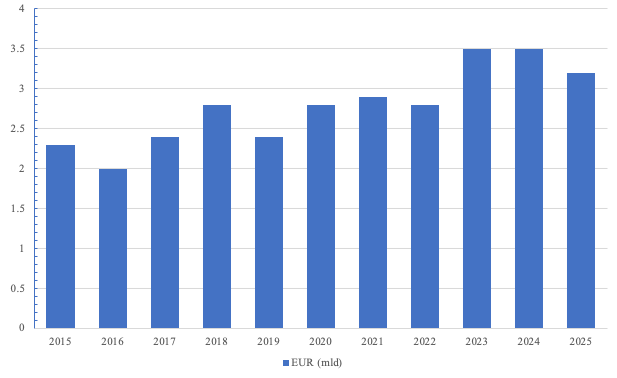
\includegraphics[height=6cm]{images/1_introduction/budget.png}
    \end{center}
    \caption{Budget for maintenance of public roads \cite{Rijksbegroting:Infrastructuur}. Budget is in billion EUR.}
    \label{fig:prm}
\end{figure}

Road maintenance is performed according to an annual cyclical process. The road owner or maintainer (i.e., state, province or municipality) initiates a tender for inspection. After which, an inspection company inspects the road with specialized vehicles. This vehicle contains multiple cameras to record the road surface, infrared sensor to measure the evenness, and other types of sensors. The recorded video data is manually inspected by engineers according the prescribed CROW method \cite{CROW_147}. The inspection company delivers a report with recommendations to the road owner indicating which roads needs maintenance. On this recommendation, the road owner initiates another tender to perform the actual maintenance. Interestingly to note is that companies that can perform inspections, often also can perform the construction.

The condition of the road is measured through various quantifiable data sources. These sources are manually inspected according to CROW method to assess the state of the road. Below is a list given of data sources which are often used within the Netherlands for road inspection:
\begin{itemize}
\item Visual inspection: video data is manually annotated to mark damages.
\item ARAN measurements: laser sensor which measures distance between the road and vehicle across the pavement, and can be used to measure the surface unevenness or rutting.
\item Ground penetrating radar: geophysical method which uses radar pulses to get an image of the subsurface by measuring the reflected signals to assess the quality of the asphalt and deeper layers, detect sinkholes and objects below the surface.
\item Falling weight deflector: similar to ground penetrating radar, but using radar pulses, a weight is dropped and reflections are measured. This method is more commonly used in civil engineering. 
\item Skid resistance: describes the force when a locked tire (i.e., a wheel that is prevented from rotating) slides along the surface. Measurements are performed by measuring the friction on the locked wheel to detect if the road is too slippery leading to aquaplaning.
\item Static data:  besides actual measurements, there is also static data on roads such as:
\begin{itemize}
\item Materials passport describing the different layers of the road. Contains information when and how a layer was constructed and which material was used.
\item Historical maintenance reports.
\item Future date of maintenance (i.e., multi-year plan). 
\item Road intensity (i.e., how many vehicles travel the road).
\end{itemize}
\end{itemize}

\subsection{AssetWorx}
\label{sec:assetworx}

Keeping track of these various sources of data is cumbersome. Although many road owners manage this data manually, there are some tools to support their workflow. These software tools are known as ``asset management software'' or ``management systems''. One of the available tools on market is Predictive Road Maintenance (PRM), a platform for data driven asset management (see figure \ref{fig:prm}) developed by AssetWorx\footnote{Pronounced as Asset Works}, where the use cases of this thesis is derived. PRM was initially developed during an incubator program known as ``Startup in Residence'' funded by the Overijssel province \cite{Residense2020}. The goal of AssetWorx is to create an uniform data platform for asset management. The idea is to be a industry disrupter by providing data driven insights concerning road quality, maintenance and planning as an independent organization. 

\begin{figure}[ht]
    \begin{center}
    \includegraphics[width=0.8\textwidth]{images/1_introduction/prm-overview.png}
    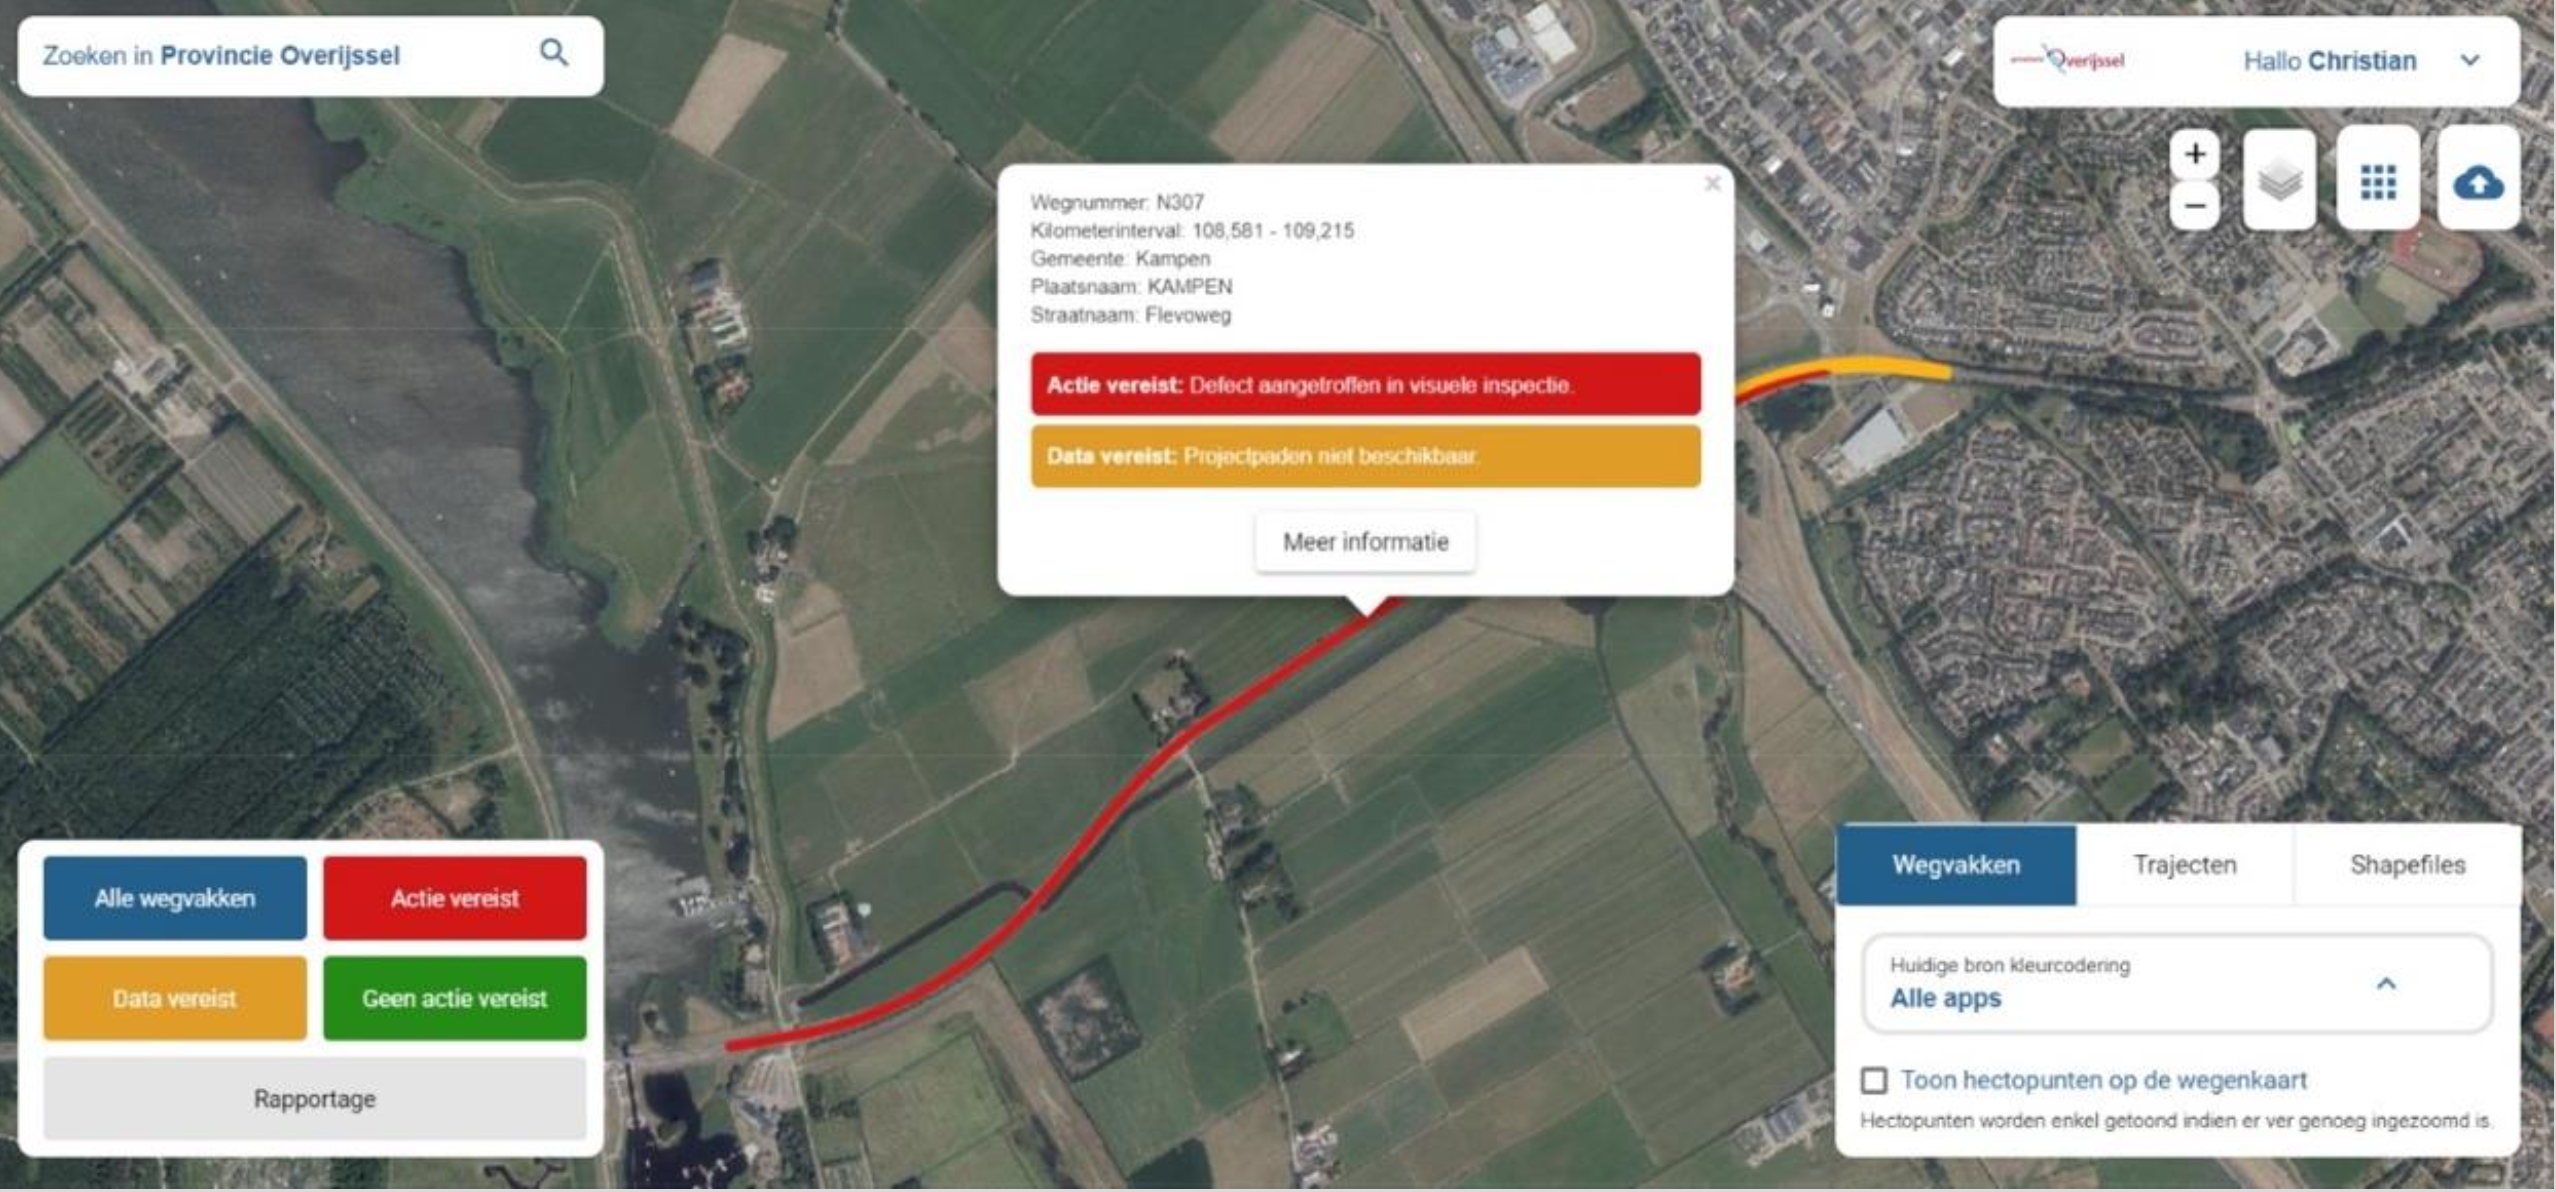
\includegraphics[width=0.8\textwidth]{images/1_introduction/prm-detail.png}
    \end{center}
    \caption{Screenshots of Predictive Road Maintenance (PRM) software.}
    \label{fig:prm}
\end{figure}


\subsection{Relevance}
\label{sec:relevance}

Although there are other asset management tools in the market, they typically only incorporate one or two data sources, mainly visual inspections. Instead, PRM is designed as a big data platform and operates on different types of data. As described beforehand, currently in Netherlands, all road assessment rely on visual inspections based on the CROW systematic \cite{CROW_147}. This procedure is intensive and largely relies on experience and inspectors' and maintainers' intuition. The cycle of tendering $\rightarrow$ inspection $\rightarrow$ tendering $\rightarrow$ maintenance, typically takes one year. However, when there is a damage in the pavement, the severity of that damage increase as it remains unrepaired. For instance, a pothole starts relatively small but over time, as more traffic passes, it can become a significant damage. Repairing a small pothole is easy and quick, but as the damages increases, so does the financial costs of repairing the road. Therefore, timely monitoring of road damages saves costs for the maintainer while increasing driving comfort and safety.

AssetWorx aims to systematically and continuously collect data of all roads instead of the conventional annual cycle of inspection and maintenance. The collected data is then processed to automatically determine the state of the road, which is the goal of this thesis. In other words, we aim at automatically detect road surface damages that  none of the existing management tools on the market can identify, although some construction companies tried to pursue this goal \cite{BAM2018}. Reaching this goal will provide a large business value for AssetWorx and for the community by reducing the cost of road maintenance.

Although automated defect detection have societal and business value, it is scientifically not something new. However, as found from literature survey, existing research only utilizes a single source of data (unimodal) to detect damages. For this research, we are collecting various types of data: camera, accelerometer, and GPS. Multimodal fusion aims to integrate data of different sources and types in a unified representation \cite{Baltrusaitis2017}. The idea is that by fusion richer information is provided than a single modality can provide. For example, damages may be detected with images, but it is difficult to assess the severity of that damage due lack of depth information. By fusing vibration data from the accelerometer, an additional dimension is added which could describe the severity of a damage. Within existing literature on road defects detection, multimodal fusion has not been applied. Fusion of accelerometer and visual data is largely researched in the context of odometry / robot navigation.

However, fusion of visual and accelerometer data proposes an interesting challenge in this context. The camera is facing towards the road, and therefore sees an object in advance at timestamp $t_{visual}$. However, at some later point the vibrations are measured at timestamp $t_{accelerometer}$. Between these sensors there is some delay $\tau$. This delay is composed of two additive delays: $\tau = \tau_{capture} + \tau_{detection}$. $\tau_{capture}$ refers to the delay between capturing visual and accelerometer data, it is expected that there is a very small delay. $\tau_{detection}$ refers to the earlier mentioned problem that an object is detected in advance, before the accelerometer measures that event. The latter delay is variable and depends on the angle of the camera, and the travelling speed.

\begin{figure}[ht]
    \begin{center}
    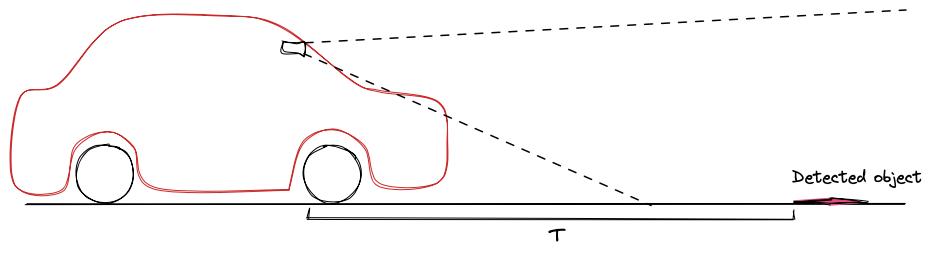
\includegraphics[width=0.95\textwidth]{images/1_introduction/setup-schema.png}
	\end{center}
    \captionsetup{width=.90\textwidth}
    \caption{Illustration of the setup of collecting data.}
    \label{fig:time-synchronization}
\end{figure}




\subsection{Research Questions}

During this research, data is continuously collected from driving on roads. In particular, it is collected by a smartphone with a customized app, which collects GPS, accelerometer, and video data that need to be combined. Visual data can only be recorded in decent conditions i.e., it depends on weather and lighting. Complementary, vibrations can always be measured regardless of external conditions. At the same time, interpreting vibration data is a more difficult task for humans. Combining both data sources helps to interpret the data. With these points in mind, this thesis aims to answer the following research question:

\begin{itemize}
\item \textbf{RQ: To what extent can visual object detection and accelerometer data be combined in a multimodal machine learning pipeline to correctly classify road surface anomalies?}
\end{itemize}

To answer this question, we divided the question into smaller parts. From quick literature survey, it is known that research exists on classifying road surface defects on single source of data. As the aim is to combine visual- and accelerometer data, it makes sense to first research what is known for each respective source in the field of road surface defect detection. Detecting defects using visual data is basically object detection: localization and classification of objects (i.e., damages) in an image. The first two sub research questions are:

\begin{itemize}
\item \textit{SQ1: What is the state of art in machine learning pipelines using object detection to classify road surface anomalies?}
\item \textit{SQ2: What is the state of art in machine learning pipelines using accelerometer data to classify road surface anomalies?}
\end{itemize}

The final answer to the RQ is evaluated based on the empirical results. When we observe that the classification accuracy of the pipeline with combined data is sufficient, we can conclude that combining both sources was successful.


\subsection{Contributions}

This thesis provides interesting contributions, both scientifically from the performed research, and business value from the developed application. First of all, this is the first research to combine both visual and accelerometer data to detect road surface anomalies. The effect of combining sources is rigorously evaluated by comparing the difference in accuracy between combined pipeline and of the respective unimodal pipelines. When the combined pipelines perform adequately we expect a higher performance than when a single data source is used. Additionally, it allows to perform classifications when only one source of data is available. 

Secondly, current asset management tools only store and organize a single source of data. When the developed model is incorporated into the PRM software, AssetWorx has a competitive advantage. Additionally, with the developed model the maintenance cycle becomes data driven and allows for quicker iterations. In turn, this means that maintainers can act quickly on damages and prevent large costs.

\subsection{Remainder}

The remainder of this thesis is structured as follows. In section \ref{sec:related-work} we describe the related work. What currently is known on detecting road surface defects using machine learning. It lays the foundation to answer the two sub research questions. Additionally, it introduces the field of multimodal machine learning. Next, section \ref{sec:background} provides background information on the used techniques. Section \ref{sec:data-processing} describes the method of collecting the data, and preprocessing steps. In section \ref{sec:experimental-design} we describe the various machine learning models that are developed. Subsequently the results of the various models are presented in section \ref{sec:results}. Next in section \ref{sec:discussion} we discuss the results and answer the various research questions. Finally, section \ref{sec:conclusion} provides a summary of the work and concludes our research.

\clearpage
\section{Literature}

\subsection{Multimodal Machine Learning}

We experience the world as multimodal: we see objects, feel vibrations and hear sounds. Modality refers to the way in which something happens or is experienced. A research problem is characterized as multimodal when it includes multiple of such modalities \cite{Baltrusaitis2017}. Commonly referred example of an interesting multimodal experience is the McGurk effect \cite{McGurk1976}. This is the perception between hearing and vision in speech. When we hear the syllable /ba/ while watching the lips of someone saying /ga/, we perceive it as /da/. 

Multimodal research has a long history from audio-visual speech recognition to more recent interest due deep learning \cite{Ngiam2011}. It has been proven that multimodal learning algorithms performs really well on various tasks, such as (audio-visual) speech recognition \cite{Noda2014}, image sentence matching \cite{Ma2015} and RGB-D object recognition \cite{Eitel2015,Xu2017,Sindagi2019}.

\authorref{Baltrusaitis2017} identified five challenges dealing with multimodal machine learning:
\begin{enumerate}
\item \textbf{Representation}: how to represent and summarize multimodal data to exploit the complementary and redundancy of multiple modalities. Distinction is made between \textit{joint representation} - which combines unimodal signals in the same space, and \textit{coordinated representation} - which processes unimodal signals separately, but enforces similarity constraints. See figure \ref{fig:structure-joint-coordinated} below for an illustration.
\item \textbf{Translation}: how to translate data from one modality to another. For example, given an image the task is to give a caption to describe the image.
\item \textbf{Alignment}: how to identify direct relations between (sub)elements from multiple modalities. For example, given an image and a caption, find the area in the image describing the caption.
\item \textbf{Fusion}: how and when to fuse / join information from multiple modalities. Historically the original topics of multimodal machine learning, with emphasize given on early-, hybrid- and late-fusion.
\item \textbf{Co-learning}: how to transfer knowledge between modalities. For example by exploiting knowledge of a rich modality, to aid modelling of a less describing modality.
\end{enumerate}

\begin{figure}[ht]
\begin{center}
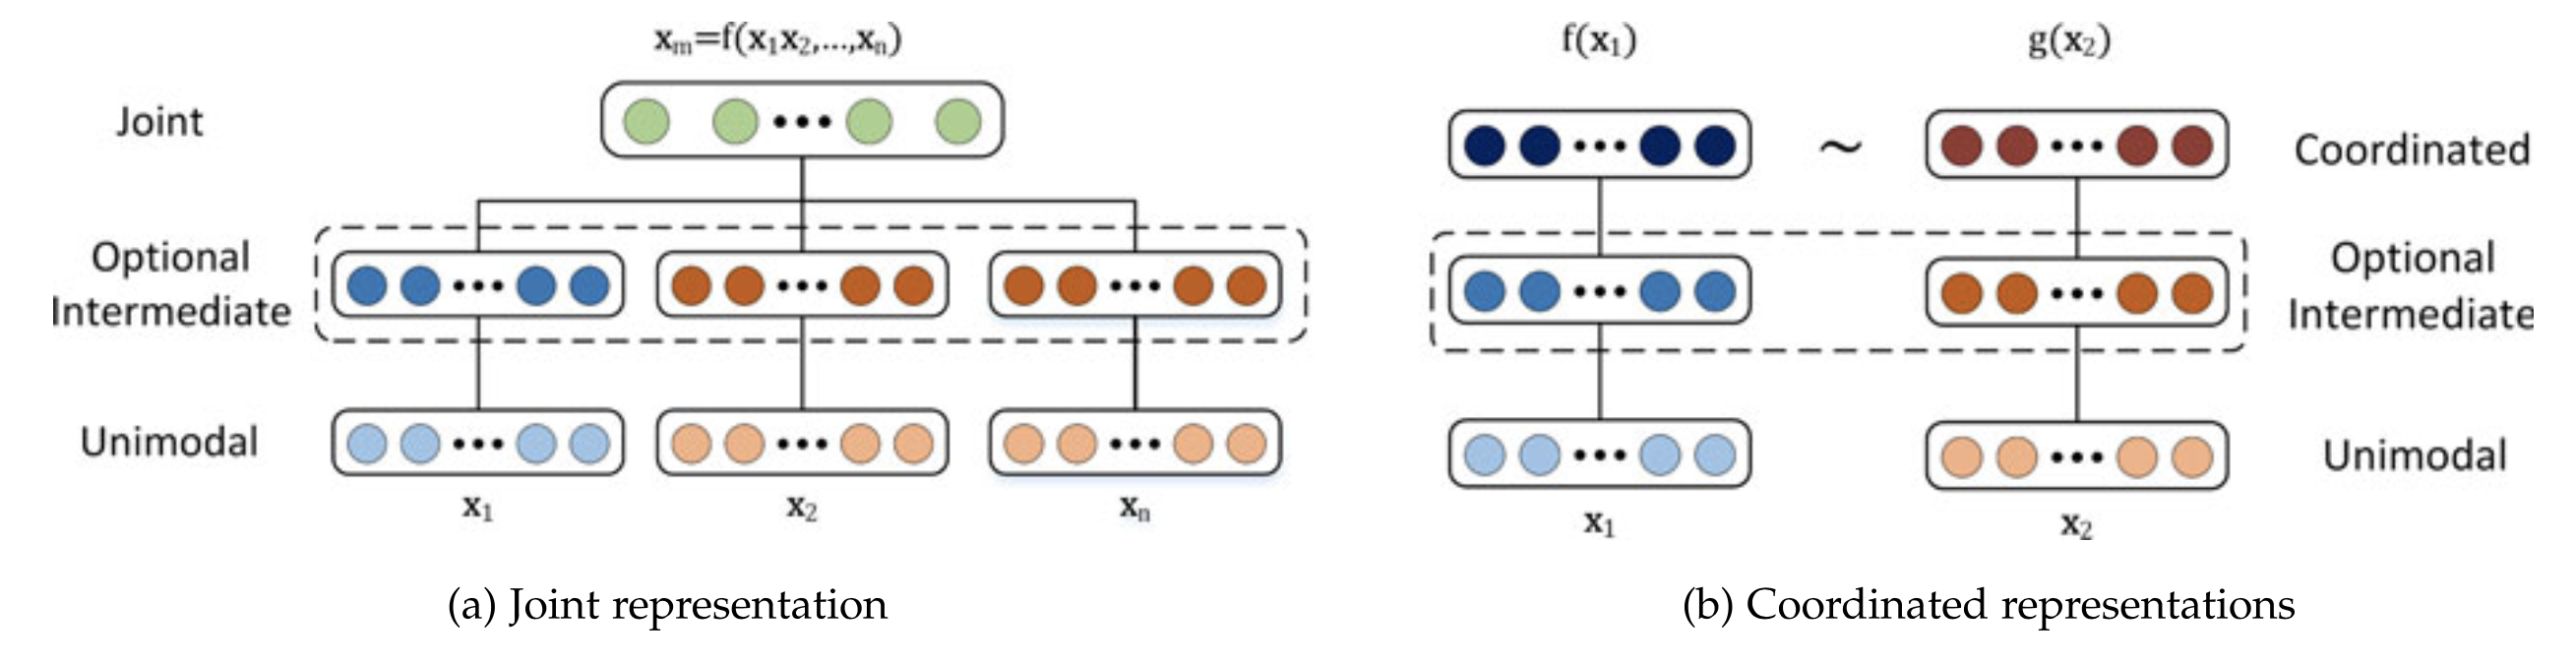
\includegraphics[width=\textwidth,keepaspectratio]{images/2_literature/joint-vs-coordinated-representations.png}
\end{center}
\caption{Structure of joint and coordinated representation \cite{Baltrusaitis2017}}
\label{fig:structure-joint-coordinated}
\end{figure}

For my thesis I think the most important challenges will be relating to representation, alignment and fusion.

To my knowledge there hasn't been any research performed on multimodal fusion on road defects. In the broader sense, multimodal fusion has been applied to detect damages. Examples of which are: combining audio-visual data to detect conveyor belt damages \cite{Che2021}, gearbox fault detection based on vibrations and acoustic signals \cite{Li2016}. See \cite{Olivan2018} for more examples of data fusion in industry.

Further exploratory research shows that visual and accelerometer (IMU) data are mainly fused in odometry. Odometry is the use of motion sensors to estimate the location over time, often used in intelligent robots. The purpose of fusing these data types is often used for dead-reckoning. Which is the process of calculating the current position based on previously known position, e.g. can be used when GPS connection is unstable / lost \cite{Jiang2017,Brossard2020}.

Although mutimodal fusion hasn't been applied to road surface defects, something related has been done by \authorref{Lekshmipathy2020}. In the paper the researchers compared the results of classifying defects based on vibrations (accelerometer) with a vision-based method. They find that vision-based method outperforms the vibration-based method. Nevertheless, they argue that vibration-based method is still useful. Vision based approach only works during daytime (under correct lighting), whereas vibrations can always be collected regardless of lighting situation or weather.

\subsubsection{Conclusion}
Although multimodal machine learning is not something new, it hasn't been applied in the domain of road maintenance. To my knowledge the fusion of accelerometer and visual data hasn't been used yet for detecting damages in general. The closest comes the work of \authorref{Lekshmipathy2020}, where they compare vibration- and visual-method for classifying road defects. My thesis aims to fill the gap by applying multimodal machine learning to detect road damages. 

% ********************************************************************************
% ********************************************************************************
% ********************************************************************************

\subsection{Automatic Road Defects Classification}

Preliminary literature review shows that there is a whole field about data driven road quality assessment. This field is driven by the fact that traditional methods of assessing road quality is costly, due requirement of specialized equipment. Researchers focuses on alternative forms to collect the data by cheaper methods, such as smartphones and sensor boxes. In current literature we identified the following \textit{subfields} based on the type of data that is used:

\begin{enumerate}
\item Road surface defects: based on image data (e.g. cracks).
\item Roughness evaluation: based on accelerometer / gyroscope (e.g. IRI).
\item Noise labelling: based on microphones.
\end{enumerate}

\begin{figure}[h!]
\begin{center}
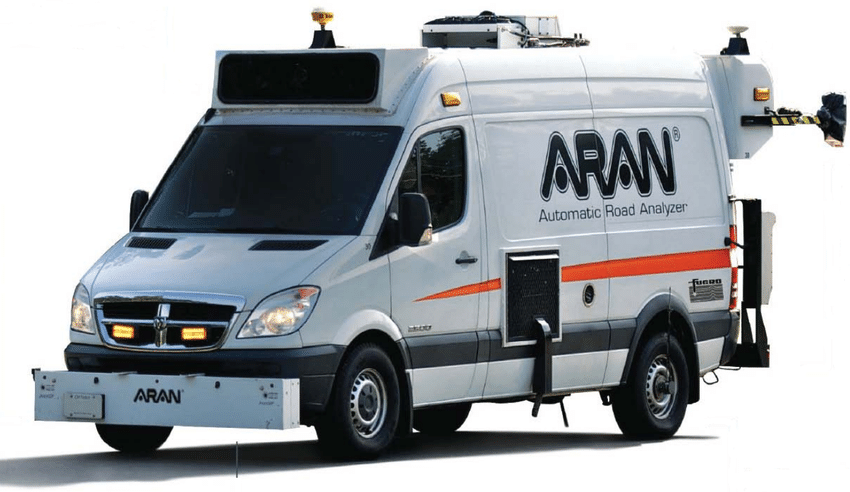
\includegraphics[height=5cm,keepaspectratio]{images/2_literature/aran.png}
\end{center}
\caption{Automatic Road Analyzer (ARAN) is specialized vehicle to gather data about the road surface \cite{Gupta2020}.}
\end{figure}

\subsubsection{Road surface defects}
Road surface defects or crack detection is a field trying to automatically classify damages based on image data. Usually the source of these images are smartphones. Additionally, there is also research performed using blackboxes (dashcams) and Kinect, where the latter is also able to measure depth. Research evolved from pictures taken from a top-down view, to front-faced view to support gathering data while driving.

In \authorref{Jahanshahi2012} the authors uses a Kinect sensor to collect image and depth data. Recording of the road has been performed from a top-faced view. The authors classify cracks, potholes and patches with accuracy scores of respective 78\%, 92\% and 90\%. By including depth measure, the problem is relatively trivial as classification is done by checking if the depth is greater than some threshold. 

\authorref{Zhang2016} proposes the first model (to their knowledge) which uses deep learning to detect road cracks. Their data has been collected by smartphones, although not mentioned explicitly, it seems their data has been collected from top-faced view and from deliberate pictures of a known defect. Related is \authorref{Zhang2017} where the authors use 3D pavement images and deep-learning network to classify road cracks. Their research is focused on acquiring pixel-level accuracy, with the aim that the model is able to tell the size and dimensions of the crack.

\authorref{Chatterjee2018} perform road crack detection on cycle roads in Germany. Their data has been collected from a front-faced view. Extensive feature extraction is performed with various computer vision based algorithms before making classifications with machine learning models. 

\authorref{Maeda2018} researched the possibilities of road damage classification by using smartphone images. Data was collected conventional smartphone holder for cars with a front-faced view while driving. They extensively collect data about Japanese roads and publishes their data and their trained model. This is also the first paper which makes distinctions between more types of road damages, such as fading line markings and distinction between lateral / longitudal cracks. The research is continued in \authorref{Arya2020-transfer}, where additional data is collected in Czech Republic and India. With the aim to see if their model is able to transfer learn on this new data. In order to further improve the published model, \authorref{Maeda2020} uses a generative adversial network to augment more data and retrain the model. Finally, a competition is held with their collected data \cite{Arya2020-competition}. The goal is to push the state of art of road damage detection forward. The competition consisted of two challenges: 1) classification (what kind of damage) and 2) detection (where is the damage). This competition yielded a model with an average F1 score of 0.67 for all classes. Greatly improving the original model, which yielded at best a F1 of 0.40 for only a single type of damage.

Besides making classifications, there has also been research focusing on segmenting the damages into crack and non-crack parts. \authorref{Dung2018} uses a fully convolutional neural network and \authorref{Bang2019} uses a encoder-decoder network.


\subsubsection{Roughness evaluation}
A different research field is centered around measuring the road roughness. Which is defined as the deviation of the surface from the true planar surface. This deviation affects vehicle dynamics and ride quality. Two methods to classify the roughness of a profile are the International Roughness Index (IRI) \cite{Sayers1986} and the International Standards Organisation (ISO) \cite{ISO8608} classification. There are various methods for measuring the profile data, typically used by road maintenance are inertial profilers. This is a device which scans the surface of the pavement with lasers to measure the distance, example of this is the Automatic Road Analyzers (ARAN) vehicle.

Research is focused on replacing these expensive devices with accelerometers, often those found in smartphones \cite{Hanson2014,Buttlar2014,Gupta2020}. Measuring the profile is done by filtering out the vertical accelerations and calculate the roughness accordingly to the IRI or ISO specification. Additionally, using the accelerometer it is also possible to identify potholes, bumps and patches \cite{Lekshmipathy2020}. 

Limitation of this method is that the accelerometers need to be calibrated, which is also deeper described in \cite{Gupta2020}. \authorref{Jeong2020} therefore argue that requirement of calibration hinders the widespread use of the technology. They propose a novel method using a convolutional neural network to eliminate the requirement of calibration.


\subsubsection{Noise labelling}
Quality of the road surface influences noise and vibrations emissions caused by the interaction between the tires and the road. In the EU, member states are required to publish noise maps for roads every five years \cite{EU2002}. Monitoring can be done with a vehicle equipped with a Close Proximity (CPX) trailer. This devices measures the emitted sounds from a reference tire.

\begin{figure}[ht]
\begin{center}
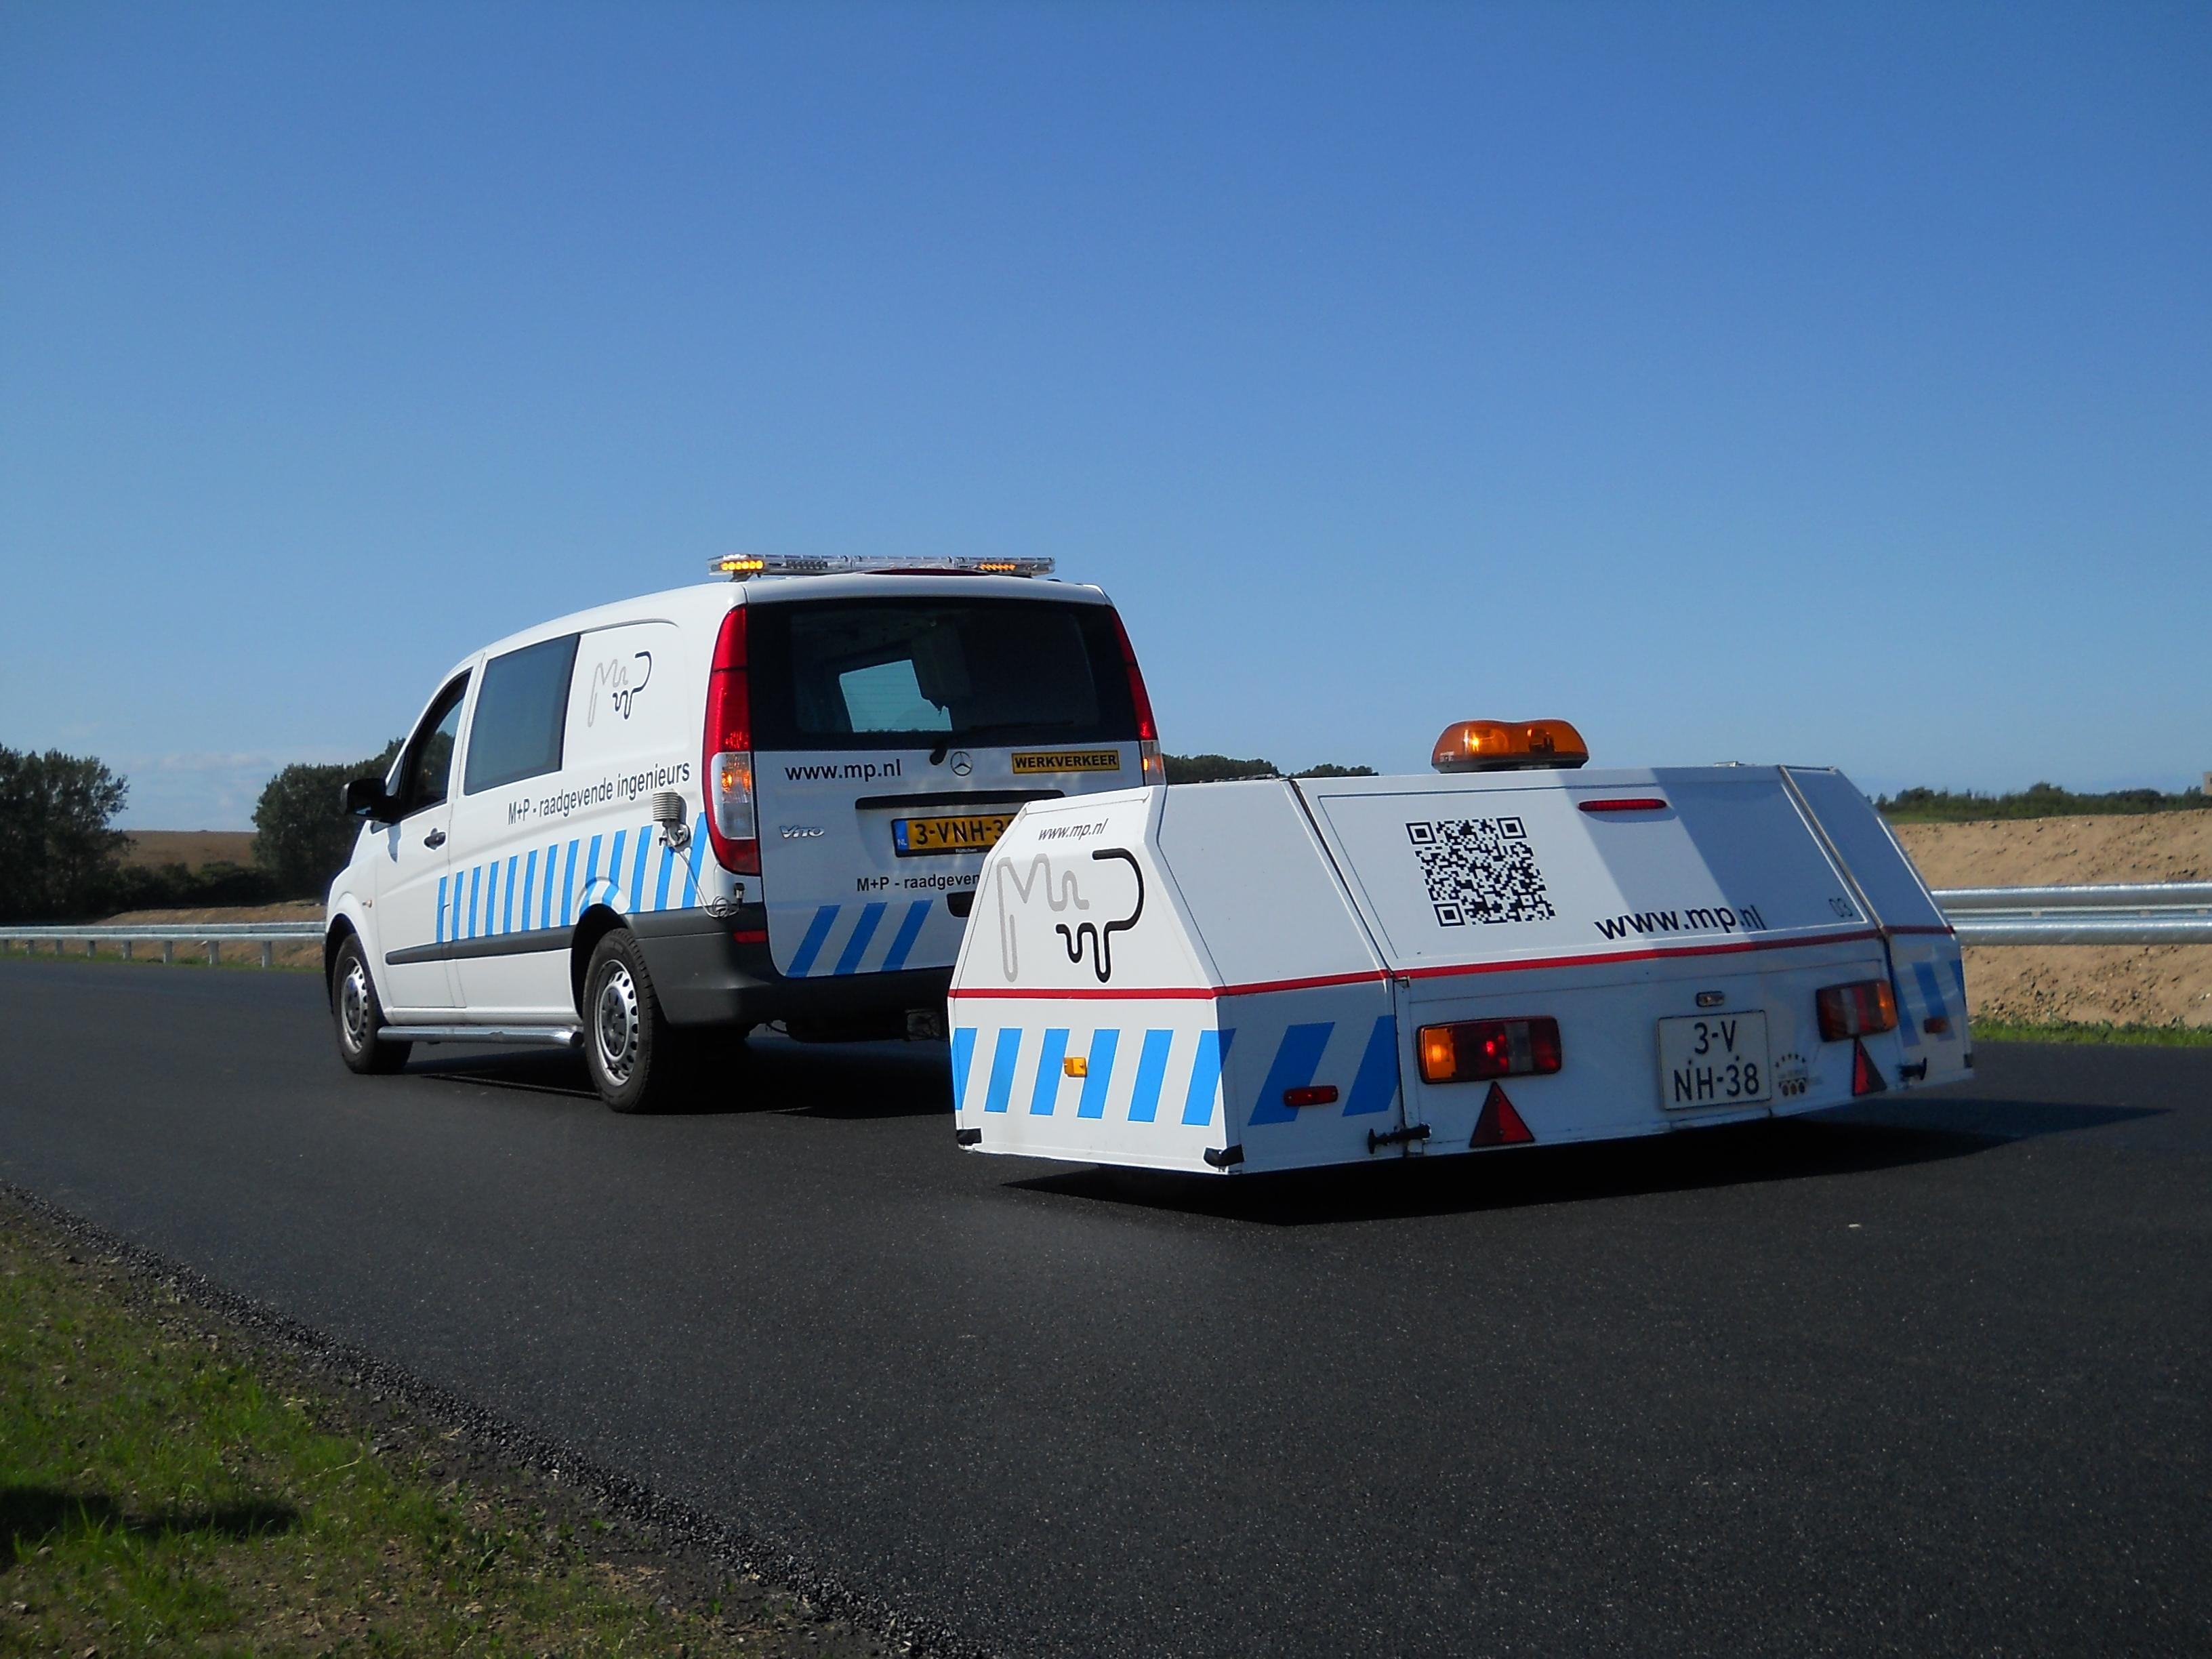
\includegraphics[height=5cm,keepaspectratio]{images/2_literature/cpx-trailer.jpg}
\end{center}
\caption{Close Proximity (CPX) trailer measures the sounds emitted by reference tyre \cite{MP2020}.}
\end{figure}

\authorref{Hauwermeiren2019} try to replicate the results of CPX measurements by using a sensor box containing a microphone. This microphone is located inside the trunk of the car. The authors were able to accurately estimate the road texture. However the with main limitation is that the data was collected under good conditions, such as no background radio or talking. This research is later continued, where the authors use multiple vehicles and more realistic driving conditions. They found that below 1600 Hz, their results differ from CPX less than the difference between bi-annually repeated measurements, indicating it is possible to perform this measurement using microphones \cite{Hauwermeiren2021}.


\subsubsection{Conclusion}
Automatic classification of road defects have been extensively researched. Main topic of interest is the usage of low-cost devices such as smartphones to collect the data. From the literature we find that only the following types of defects are classified: cracks, patches, holes and faded line markings. Raveling, rutting and skewed signs haven't been researched yet to my knowledge. From the field of classifying road defects we can draw a lot of knowledge to use for my thesis. Especially this is useful when to model the right representations of the data to use for multimodal machine learning.

% ********************************************************************************
% ********************************************************************************
% ********************************************************************************

\subsection{Object Detection}

% ********************************************************************************
% ********************************************************************************
% ********************************************************************************

\subsection{Accelerometer Signal Processing}

% ********************************************************************************
% ********************************************************************************
% ********************************************************************************

\subsection{Alignment of Sources in Multimodal Fusion}
\clearpage
\section{Research Methodology}

The final solution for the company is a model to assess road quality based on different sources of data. Methodologically we can see this as a design problem. In which the research goal is to design, develop and evaluate an artefact (solution)\cite{Hevner2004}. In order to ensure a certain degree of scientific rigor, a design science methodology is used \cite{Versloot2019}.

In this respect Hevner et al. \cite{Hevner2004} is commonly referred to, in which researches perform cyclical process of development and evaluation. However, Sein et al. \cite{Sein2011} state that traditional design research has drawbacks in which scientific rigor is more valued than organizational value. Thereby failing to recognize that the artefact actually emerges from interaction with the organization. In their paper, the authors propose a new method called Action Design Research (ADR). This method based on a more iterative approach. This approach reflects the premise that IT artefacts are shaped by the organization, both during development and use. It conceptualizes research process as the interwoven activities of: building the IT artefact, intervening in the organization and evaluating it concurrently \cite{Sein2011}.

ADR consists of the following four stages \cite{Sein2011}.
\begin{enumerate}
\item \textbf{Problem Formulation}: identifies and conceptualizes a research opportunity. The trigger is a problem perceived or anticipated by the researchers. Input can come from practitioners, end-users, researchers, existing technology and/or review of prior research.
\item \textbf{Building, Intervention, and Evaluation}: iterative process which interweaves building the IT artefact, intervention in the organization, and evaluation (BIE). The problem framing of stage one is used to generate an initial design of the IT artefact which is further shaped by organizational use and subsequent design cycles. During BIE, the problem and artefact are continually evaluated.
\item \textbf{Reflection and Learning}: recognizes that the research problem involves more than simply solving a problem. Conscious reflection on the problem framing, theories chosen, and the emerging ensemble is critical to ensure contributions to knowledge are identified. This is a continuous stage which run in parallel with the first two stages.
\item \textbf{Formalization of Learning}: has the goal to generalize the learning. Making the learning from specific-and-unique to a generic-and-abstract. 
\end{enumerate}

This thesis proposal states the problem formulation that road quality assessment is a costly and labor-intensive procedure (see section \ref{section:problem}). On approval of this proposal we'll move to the following stages. \textit{Building, Intervention, and Evaluation} is the experimental process in which the activities from above are performed. This stage will be done in accordance with the organization. With the purpose to make artefacts in such way that they are usable by the organization. The following stage \textit{Reflection and Learning} is done in accordance with the university of which the contributions and learnings are written down in my thesis. Finally the stage \textit{Formalization of Learning} will be done in the discussion and reflection of my thesis.

\clearpage
\section{Data Collection and Processing}


\clearpage
\section{Multimodal Machine Learning}


\subsection{General Experiment Setup}
Experiments in subsequent sections are all ran on the same machine. This machine has the following specifications: Intel Core i7-7700K CPU, NVIDIA GeForce GTX 1080 GPU and 32 GiB RAM. Experiments are tracked with an open-source tool called Weights and Biases (wandb) \cite{wandb}.

TODO: frame experiments as Action Design Research cycles


\subsection{ADR Cycle 1: Detecting Roadside Location Markers}

With object detection the evaluation metrics measure how close the detected bounding boxes are to the ground-truth (labelled) bounding boxes. This measurement is done independently for each object class, by assessing the amount of overlap. Models are assessed on the following metrics: precision, recall and mAP \cite{Padilla2021}.

Precision is ability to identify only relevant objects, the percentage of correct predictions. Recall is ability to find all relevant cases, the percentage of correct predictions among all given ground truths. In practice, we want a good object detector that find all ground truth objects (high recall), while only identifying relevant objects (high precision). Average Precision (MP) is metric based on the area below Precision x Recall curve. AP is obtained for each individual class, to yield a single metric, mean average precision (mAP) can be calculated by averaging the AP over all classes \cite{Padilla2021}.

TODO: describe mAP calculation

The first experiment is to detect roadside location markers, also known as \textit{hectometerpaal} or \textit{mile marker}. These are  small signs that are along the road to indicate the current position. See also figure \ref{fig:road-indicator} for an example of Dutch road location marker. The task is to detect the location and orientation of road indicators from the gathered data. With this output we can determine if the road location marker is in good condition, e.g. it is not skewed backwards but clearly visible.

\begin{figure}[ht]
\begin{center}
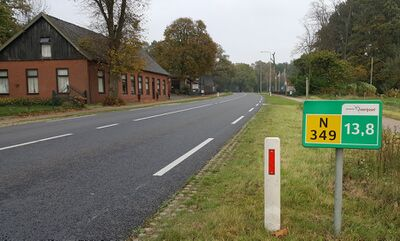
\includegraphics[height=4cm,keepaspectratio]{images/5_multimodal_fusion/example_hectometer.jpeg}
\end{center}
\caption{Example of roadside location marker (\textit{hectometerpaal}).}
\end{figure}


The reasons for this experiment are two-fold. First, the automation of detecting road sign damages. For road maintainers this is an easy optimization in their efficiency and thereby saves the road maintainers money. Second, although this is a relatively simple experiment, it enables the author to learn more about the practicalities of using YOLO, such as transfer learning, experiment tracking and resource utilization.


\subsubsection{Setup}
Classifying and locating objects is known as object detection. The output is the bounding box and class of the detected objects in an image. See also \ref{object-detection} for more information. Current state-of-the-art model for object detection is YOLOv5. This experiment uses YOLOv5 as model with pre-trained weights. The model is transfer learned to detect road side location markers. 

At this time there were 536 annotated frames with visible roadside location markers. The data comes from three different trips, filmed with the same camera. The frames are split into a training, validation and test split. With respective proportions of 70\% / 21\% / 9\%. 


\subsubsection{Results}
The following configurations are tested:


\begin{table}[h]
\begin{tabular}{lllllll}
Name                        & Model       & Image Size & Batch Size & Precision & Recall & mAP  \\
last\_95\_img-640\_batch-42 & UCS-InfoLab & 640        & 4          & 0.74      & 0.55   & 0.62 \\
yolo5m\_batch-640\_batch-4  & YOLOv5m     & 640        & 4          & 0.87      & 0.93   & 0.93 \\
yolo5s\_batch-640\_batch-32 & YOLOv5s     & 640        & 32         & 0.59      & 0.61   & 0.56 \\
yolo5s\_batch-640\_batch-16 & YOLOv5s     & 640        & 16         & 0.68      & 0.71   & 0.74 \\
yolo5s\_batch-640\_batch-8  & YOLOv5s     & 640        & 8          & 0.80      & 0.78   & 0.86 \\
yolo5s\_batch-1280\_batch-8 & YOLOv5s     & 1280       & 8           & \textbf{0.91} & \textbf{0.94} & \textbf{0.95}
\end{tabular}
\end{table}


\begin{figure}[h]
\begin{center}
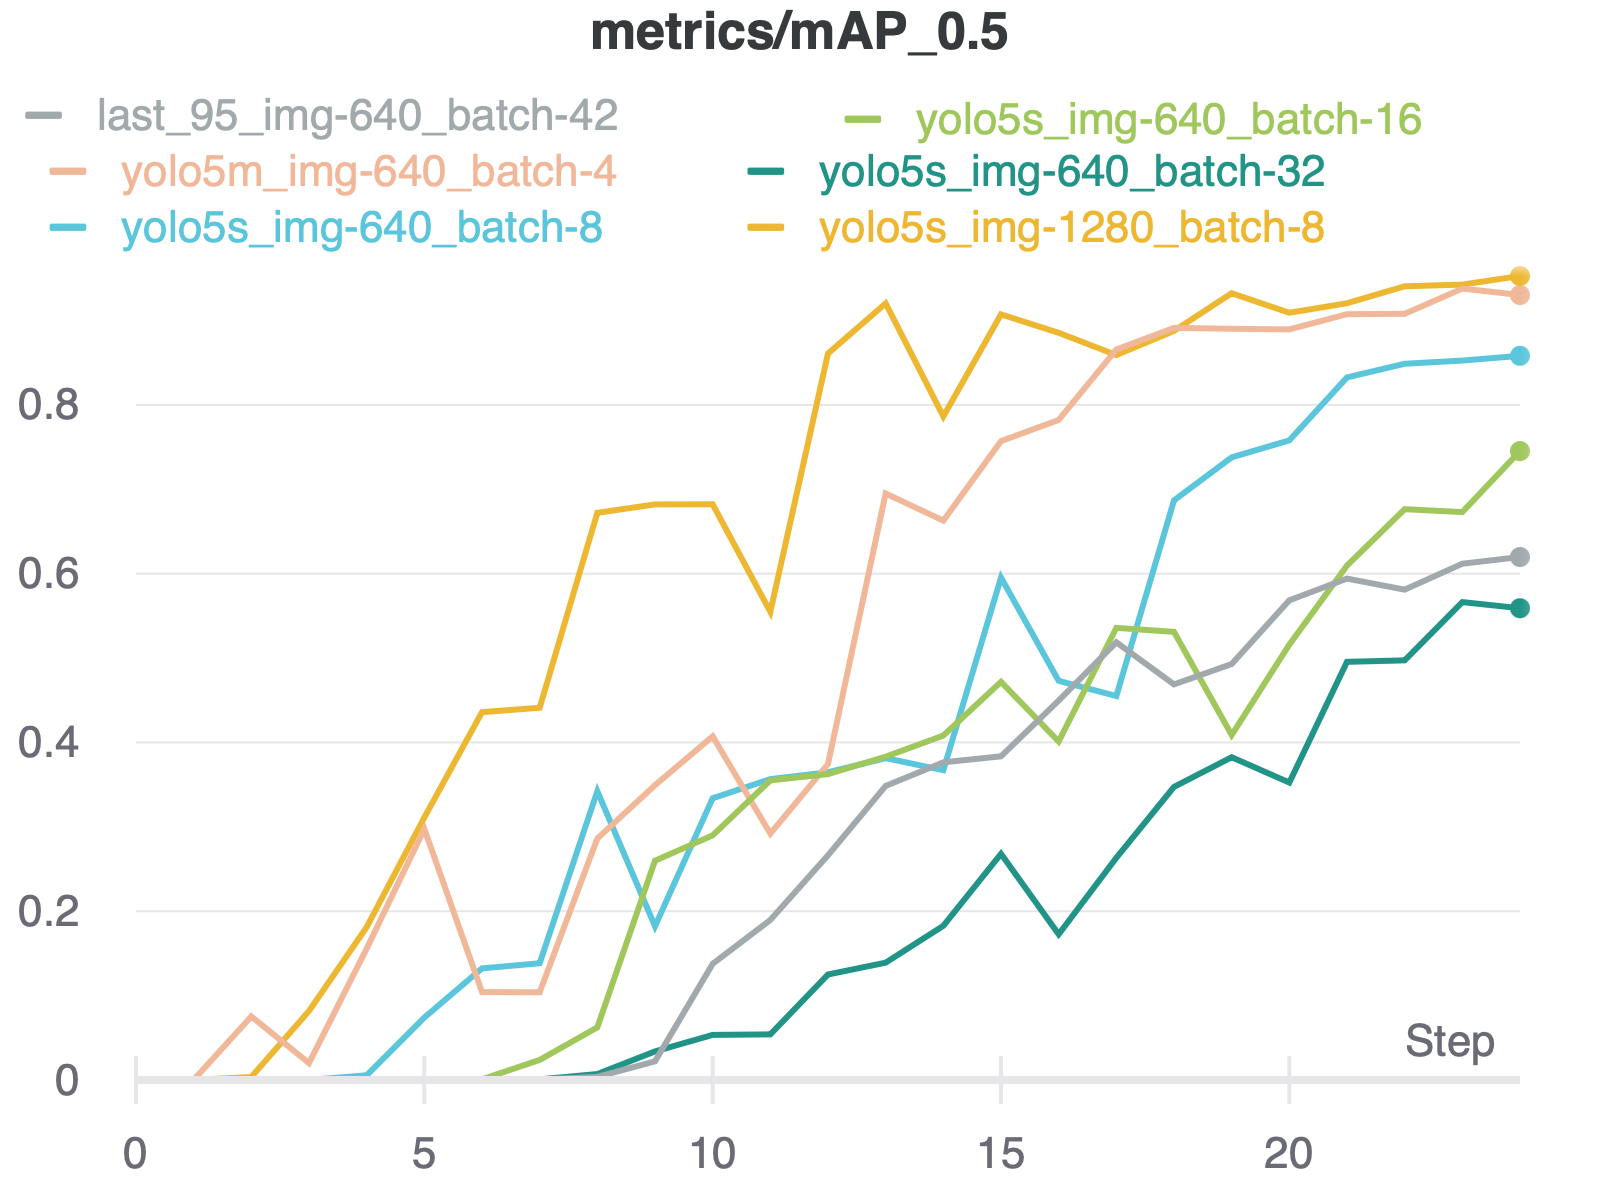
\includegraphics[height=4cm,keepaspectratio]{images/5_multimodal_fusion/exp-1_mAP.png}
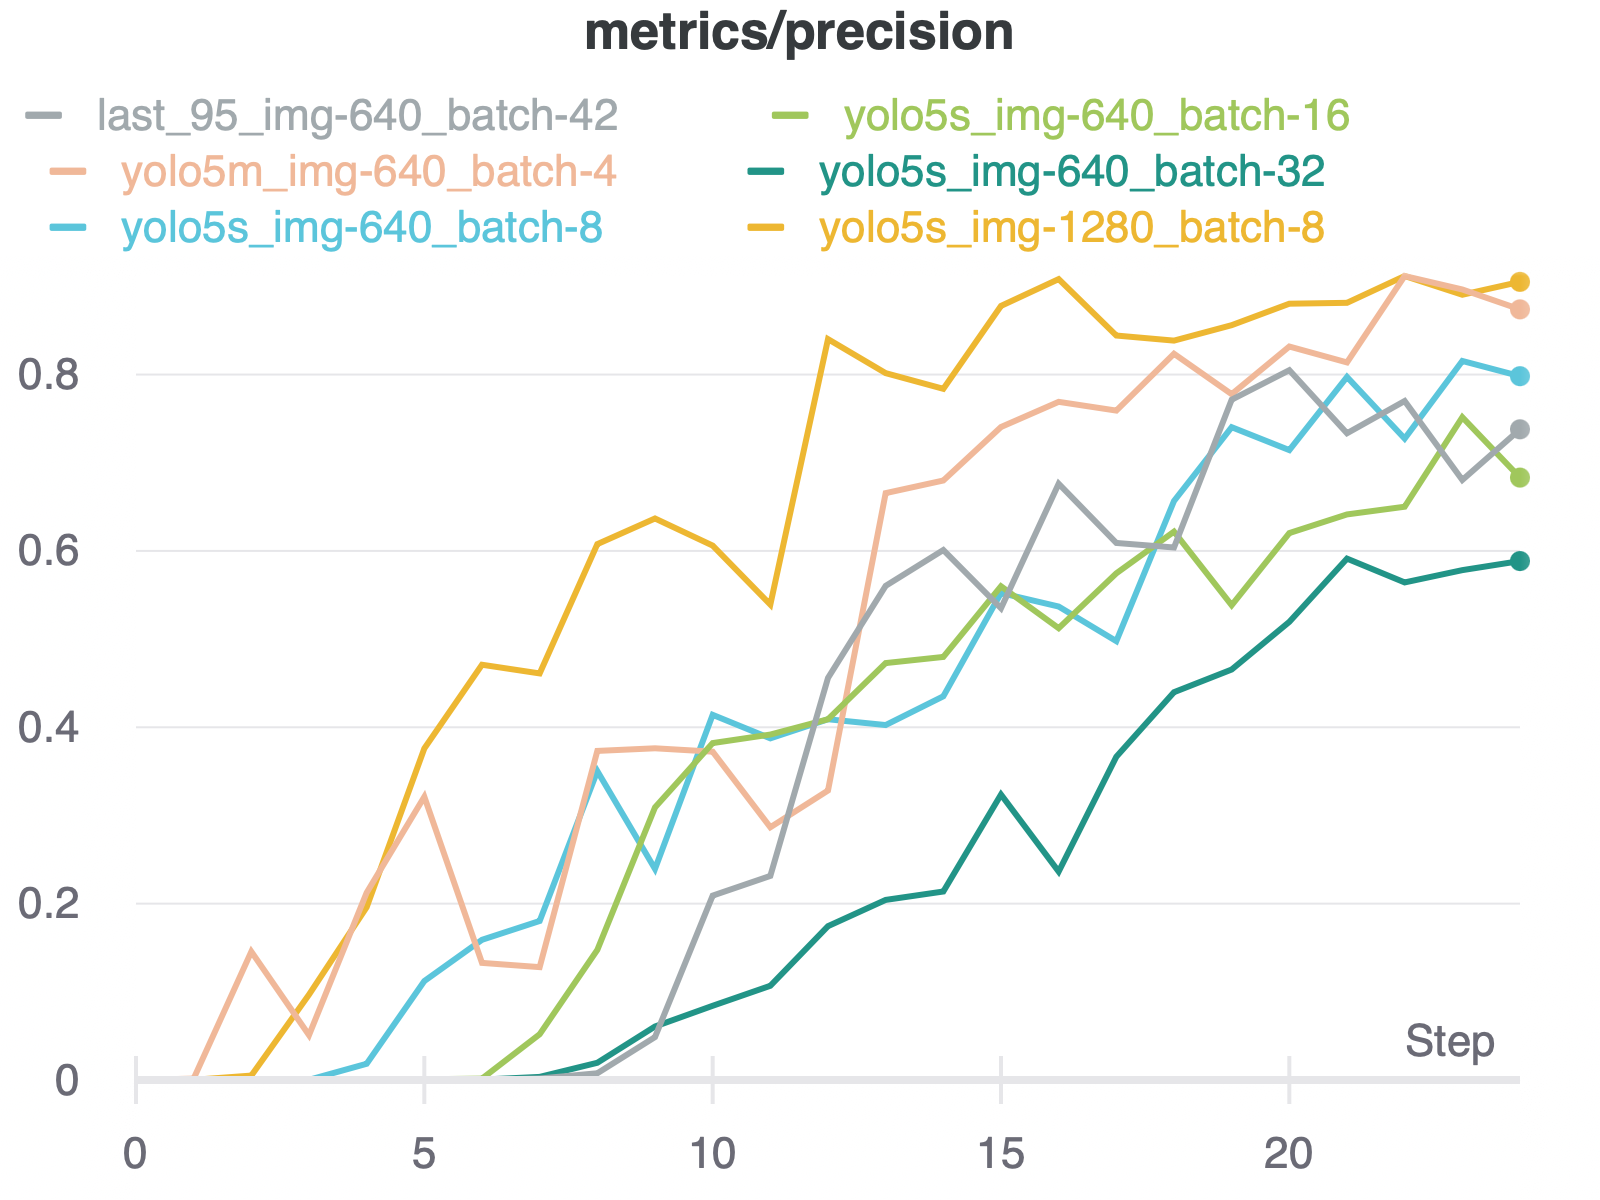
\includegraphics[height=4cm,keepaspectratio]{images/5_multimodal_fusion/exp-1_precision.png}
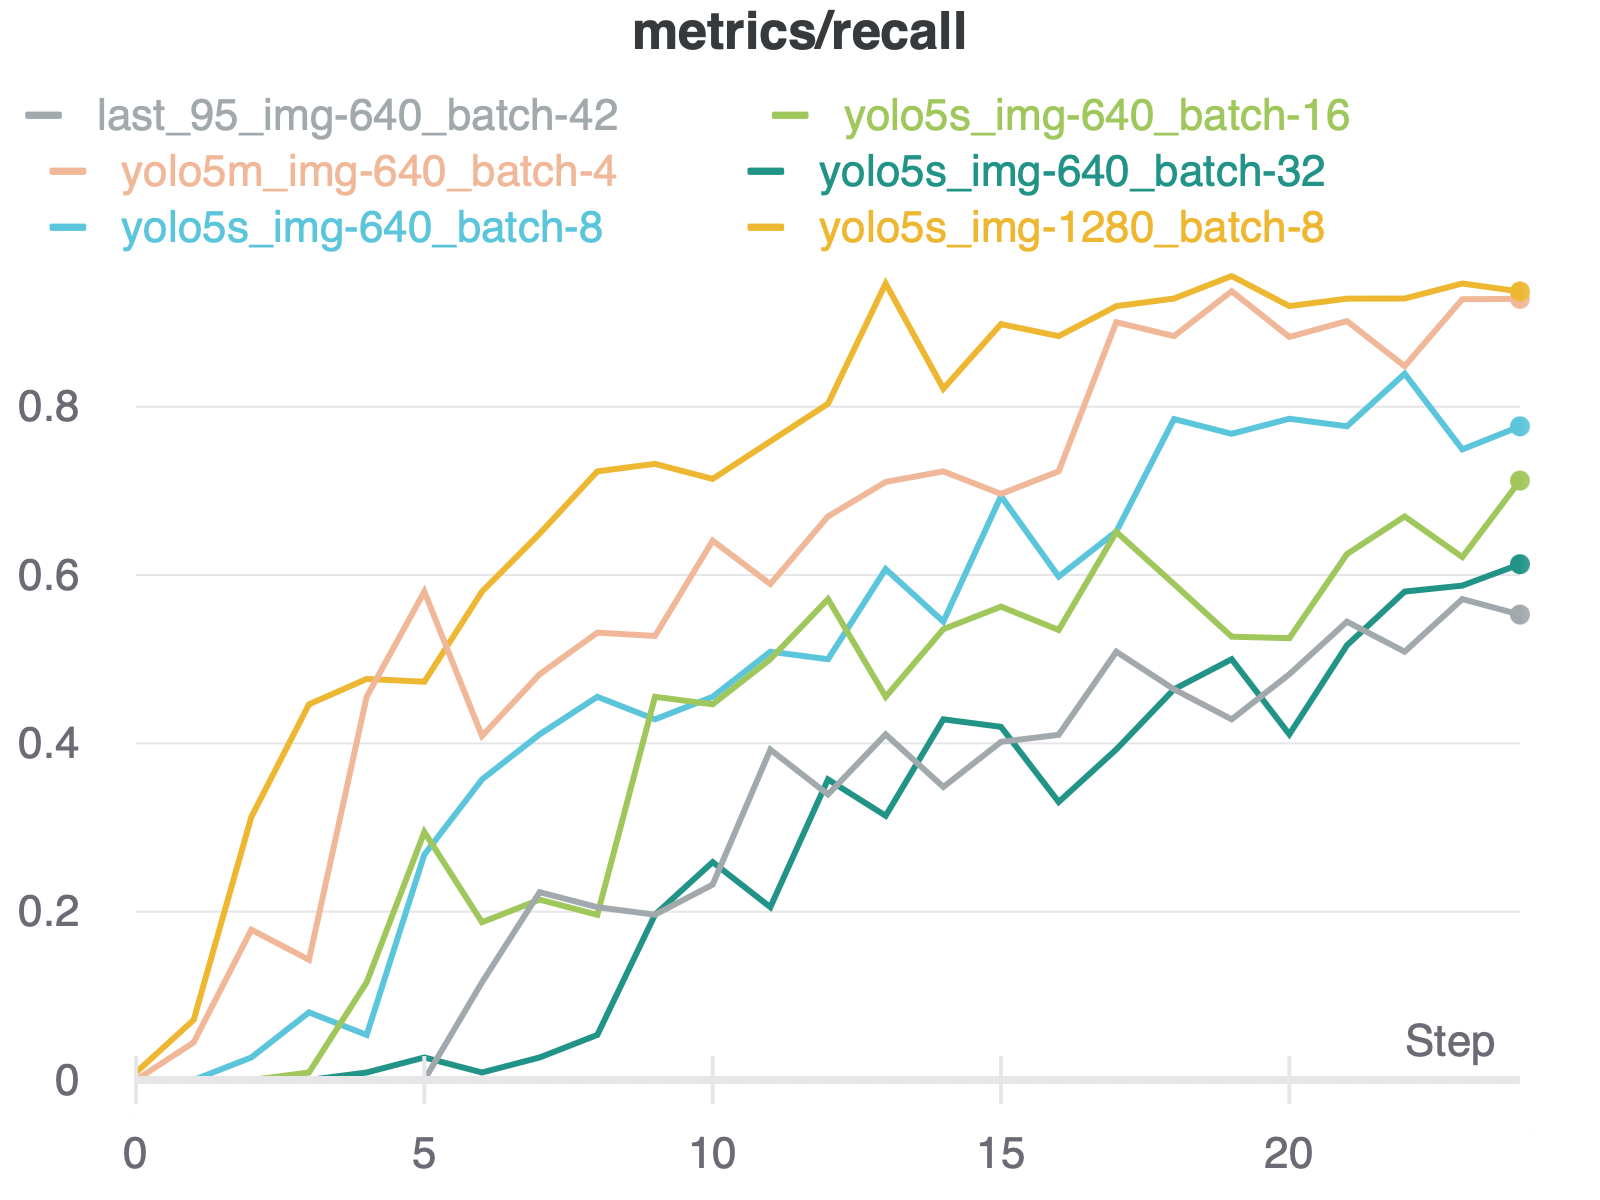
\includegraphics[height=4cm,keepaspectratio]{images/5_multimodal_fusion/exp-1_recall.png}
\end{center}
\caption{Experiment 1: performance metrics for detecting roadside location markers.}
\end{figure}


\textit{TODO: Describe the mislabelling and lower (omitted) mAP @ 0.5 scores}

\begin{figure}[h]
\begin{center}
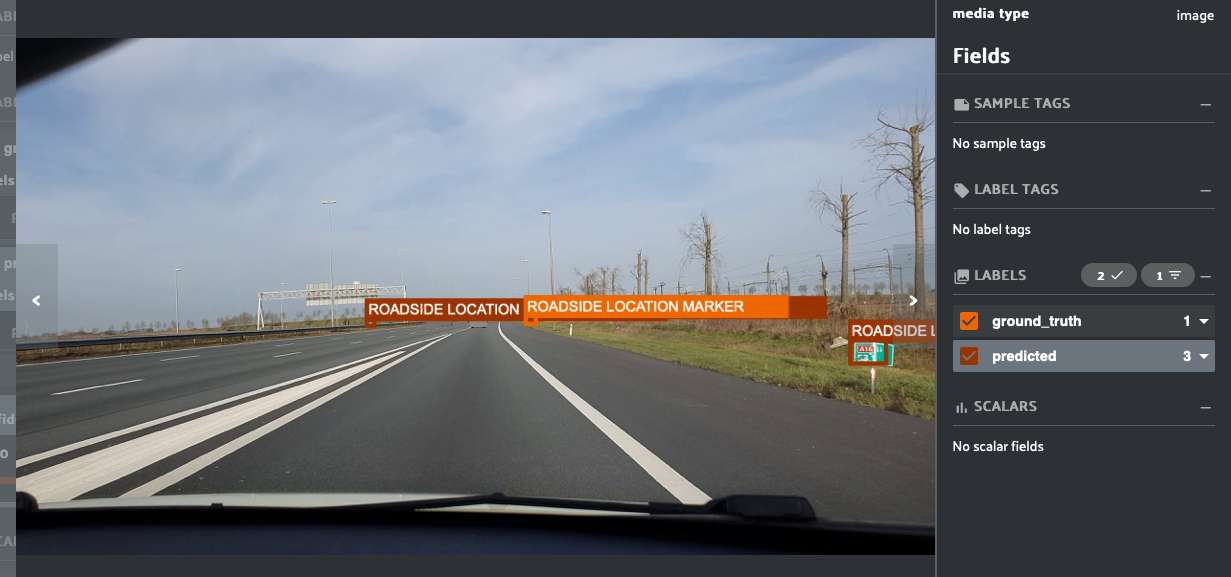
\includegraphics[width=\textwidth,keepaspectratio]{images/5_multimodal_fusion/exp-1_sample.png}
\end{center}
\caption{Example of predicted bounding boxes. Predicted boxes are in dark brown, while the ground truth labelling is in orange.}
\end{figure}

\subsubsection{Conclusion}

Detecting roadside location markers appears to be a relatively easy task for YOLO. From the results table above we see that larger models perform better. In our task this seems explainable. The roadside location marker is relatively small in the whole image. Thus, a model with larger image size works best to detect these small objects.

Although it is a simple experiment, during tests it appeared that the GPU might be a limiting factor for testing really large models. For completion, the aim was to test all possible configurations with YOLOv5s, YOLOv5m and image sizes in [640, 1280], and batch sizes in [4, 8, 16, 32]. Upon testing larger models (e.g. YOLOv5Mm with image size 1280), unfortunately the GPU experienced out of memory issues.


\subsection{ADR Cycle 2: Estimate Vehicle-to-Object Distance }

\subsection{ADR Cycle 3: Synchronize Visual and Accelerometer}

\subsection{ADR Cycle 4: Train End-to-End Multimodal DL Model}









\clearpage
\section{Discussion}
\clearpage
\section{Conclusion}
\clearpage

\section{References}

\printbibliography[nottype=online, heading=subbibnumbered, title={Scientific Articles}]
\printbibliography[type=online, heading=subbibnumbered, title={Other Articles}]



\end{document}